\documentclass[11pt,a4paper,oneside]{article}
\usepackage[UTF8,adobefonts]{ctex}

\usepackage{wrapfig}
\usepackage{indentfirst}
\usepackage{amsmath}
\usepackage{float}
\usepackage{ulem}

\usepackage[top=1in,bottom=1in,left=1.25in,right=1.25in]{geometry}

\usepackage{color}
\usepackage{xcolor}

\usepackage{multirow}
\usepackage{amssymb}
\usepackage{graphicx}

\usepackage{diagbox}
\usepackage{slashbox}
\begin{document}
\section*{五、实验数据处理}
\subsection*{1.标准状态:灯丝电源电压3.3v,$V_{G1K}$电压1.5v,$V_{G2A}$电压8.0v,$V_{G2K}$电压82v}
\begin{center}
\begin{tabular}{|c|c|c|c|c|c|c|}
	\hline
	波峰&V1&V2&V3&V4&V5&V6
	\\\hline
	电压/V&21.0&30.5&41.5&52.5&64.5&76.5\\\hline
	\end{tabular}
	\end{center}

$$  \bar{V_0}=\frac{V_4+V_5+V_6-V_3-V_2-V_1}{3\times 3}=11.17V $$
$$	\Delta V_1=\frac{1}{3}(V_4-V_1)=10.50V $$
$$	\Delta V_2=\frac{1}{3}(V_5-V_2)=11.33V $$
$$	\Delta V_3=\frac{1}{3}(V_6-V_3)=11.67V $$ 

\ \\
A类不确定度:
$$	u_a(V_0)=\sqrt{\frac{\sum\limits_{i=1}^{3} (\Delta V_i-\bar{V_0})^2}{3\times 2}}=0.347V $$
B类不确定度:
$$	u_b(V_0)=\frac{0.1V}{\sqrt{3}}=0.058V $$
不确定度:
$$	u(V_0)=\sqrt{u_a(V_0)_2+u_b(V_0)_2}=0.35V $$
相对不确定度:
$$	\eta=\frac{u(V_0)}{V_0}=0.032 $$
最终结果为:
$$	V_0 \pm u(V_0) = (11.17 \pm 0.35)V $$


\subsection*{2.灯丝电源电压改变为$3.4$v}
\begin{center}
\begin{tabular}{|c|c|c|c|c|c|c|}
	\hline
	波峰&V1&V2&V3&V4&V5&V6
	\\\hline
	电压/V&22.0&31.0&41.5&52.5&64.5&76.5\\\hline
	\end{tabular}
	\end{center}

$$  \bar{V_0}=\frac{V_4+V_5+V_6-V_3-V_2-V_1}{3\times 3}=11.00V $$
$$	\Delta V_1=\frac{1}{3}(V_4-V_1)=10.17V $$
$$	\Delta V_2=\frac{1}{3}(V_5-V_2)=11.17V $$
$$	\Delta V_3=\frac{1}{3}(V_6-V_3)=11.67V $$ 

\ \\
A类不确定度:
$$	u_a(V_0)=\sqrt{\frac{\sum\limits_{i=1}^{3} (\Delta V_i-\bar{V_0})^2}{3\times 2}}=0.441V $$
B类不确定度:
$$	u_b(V_0)=\frac{0.1V}{\sqrt{3}}=0.058V $$
不确定度:
$$	u(V_0)=\sqrt{u_a(V_0)_2+u_b(V_0)_2}=0.44V $$
相对不确定度:
$$	\eta=\frac{u(V_0)}{V_0}=0.040 $$
最终结果为:
$$	V_0 \pm u(V_0) = (11.00 \pm 0.44)V $$


\subsection*{3.$V_{G1K}$ 电压改变为$1.7$v}
\begin{center}
\begin{tabular}{|c|c|c|c|c|c|c|}
	\hline
	波峰&V1&V2&V3&V4&V5&V6
	\\\hline
	电压/V&21.0&30.5&41.5&52.5&64.0&76.5\\\hline
	\end{tabular}
	\end{center}

$$  \bar{V_0}=\frac{V_4+V_5+V_6-V_3-V_2-V_1}{3\times 3}=11.11V $$
$$	\Delta V_1=\frac{1}{3}(V_4-V_1)=10.50V $$
$$	\Delta V_2=\frac{1}{3}(V_5-V_2)=11.17V $$
$$	\Delta V_3=\frac{1}{3}(V_6-V_3)=11.67V $$ 

\ \\
A类不确定度:
$$	u_a(V_0)=\sqrt{\frac{\sum\limits_{i=1}^{3} (\Delta V_i-\bar{V_0})^2}{3\times 2}}=0.338V $$
B类不确定度:
$$	u_b(V_0)=\frac{0.1V}{\sqrt{3}}=0.058V $$
不确定度:
$$	u(V_0)=\sqrt{u_a(V_0)_2+u_b(V_0)_2}=0.34V $$
相对不确定度:
$$	\eta=\frac{u(V_0)}{V_0}=0.031 $$
最终结果为:
$$	V_0 \pm u(V_0) = (11.11 \pm 0.34)V $$


\subsection*{4.$V_{G2A}$ 电压改变为10v}
\begin{center}
\begin{tabular}{|c|c|c|c|c|c|c|}
	\hline
	波峰&V1&V2&V3&V4&V5&V6
	\\\hline
	电压/V&22.5&32.0&42.5&54.0&65.5&77.5\\\hline
	\end{tabular}
	\end{center}

$$  \bar{V_0}=\frac{V_4+V_5+V_6-V_3-V_2-V_4}{3\times 3}=11.11V $$
$$	\Delta V_1=\frac{1}{3}(V_4-V_1)=10.50V $$
$$	\Delta V_2=\frac{1}{3}(V_5-V_2)=11.17V $$
$$	\Delta V_3=\frac{1}{3}(V_6-V_3)=11.67V $$ 

\ \\
A类不确定度:
$$	u_a(V_0)=\sqrt{\frac{\sum\limits_{i=1}^{3} (\Delta V_i-\bar{V_0})^2}{3\times 2}}=0.338V $$
B类不确定度:
$$	u_b(V_0)=\frac{0.1V}{\sqrt{3}}=0.058V $$
不确定度:
$$	u(V_0)=\sqrt{u_a(V_0)_2+u_b(V_0)_2}=0.34V $$
相对不确定度:
$$	\eta=\frac{u(V_0)}{V_0}=0.031 $$
最终结果为:
$$	V_0 \pm u(V_0) = (11.11 \pm 0.34)V $$

\iffalse
\begin{comment}
\begin{figure}[H]
	\centering
		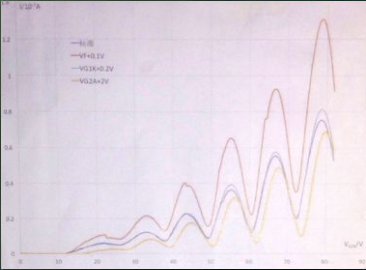
\includegraphics{lab2151_1.png}
    \caption{四条曲线对比图(仅供参考,实际图片请根据实验数据自行绘制)}
	\end{figure}

\subsection*{5.示波器自动测量}

\begin{figure}[H]
	\centering
		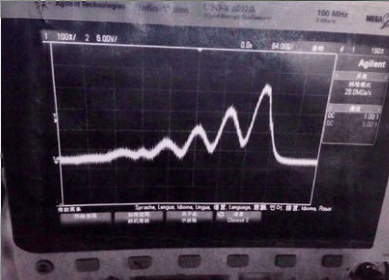
\includegraphics{lab2151_2.png}
	\end{figure}

\end{comment}
\fi
\end{document}